\documentclass[11pt,a4paper]{article}

% ====================================================================
% Packages
% ====================================================================
\usepackage[utf8]{inputenc}
\usepackage[T1]{fontenc}
\usepackage{amsmath,amssymb,amsthm}
\usepackage{mathtools}
\usepackage{hyperref}
\usepackage[margin=1in]{geometry}
\usepackage{enumitem}
\usepackage{booktabs}
\usepackage{listings}
\usepackage{xcolor}
\usepackage{cleveref}
\usepackage{mdframed}
\usepackage{tikz}
\usetikzlibrary{decorations.pathmorphing,arrows.meta,positioning,calc}

% ====================================================================
% Theorem environments
% ====================================================================
\theoremstyle{plain}
\newtheorem{theorem}{Theorem}[section]
\newtheorem{lemma}[theorem]{Lemma}
\newtheorem{proposition}[theorem]{Proposition}
\newtheorem{corollary}[theorem]{Corollary}

\theoremstyle{definition}
\newtheorem{definition}[theorem]{Definition}
\newtheorem{remark}[theorem]{Remark}

% ====================================================================
% Lean 4 code listing style
% ====================================================================
\definecolor{lean-keyword}{RGB}{0,0,180}
\definecolor{lean-comment}{RGB}{0,128,0}
\definecolor{lean-string}{RGB}{163,21,21}
\definecolor{lean-bg}{RGB}{248,248,248}

\lstdefinelanguage{lean4}{
  keywords={theorem,lemma,def,class,instance,import,open,variable,
            noncomputable,section,namespace,end,where,let,have,show,
            intro,obtain,use,exact,rw,simp,apply,by,fun,match,if,
            then,else,do,return,axiom,abbrev,private,attribute,
            suffices,change,congr,ext,constructor,rintro,push_neg,
            linarith,absurd,set_option,omit,in,set,cases,refine,
            calc,nlinarith,positivity,structure},
  sensitive=true,
  morecomment=[l]{--},
  morecomment=[s]{/-}{-/},
  morestring=[b]",
  morestring=[b]',
}

\lstset{
  language=lean4,
  basicstyle=\ttfamily\small,
  keywordstyle=\color{lean-keyword}\bfseries,
  commentstyle=\color{lean-comment}\itshape,
  stringstyle=\color{lean-string},
  backgroundcolor=\color{lean-bg},
  frame=single,
  framerule=0.5pt,
  breaklines=true,
  breakatwhitespace=true,
  tabsize=2,
  showstringspaces=false,
  numbers=left,
  numberstyle=\tiny\color{gray},
  numbersep=5pt,
  xleftmargin=15pt,
  captionpos=b,
}

% ====================================================================
% Macros
% ====================================================================
\newcommand{\NN}{\mathbb{N}}
\newcommand{\ZZ}{\mathbb{Z}}
\newcommand{\QQ}{\mathbb{Q}}
\newcommand{\RR}{\mathbb{R}}
\newcommand{\CC}{\mathbb{C}}
\newcommand{\BISH}{\mathrm{BISH}}
\newcommand{\CRM}{\mathrm{CRM}}
\newcommand{\LPO}{\mathrm{LPO}}
\newcommand{\WLPO}{\mathrm{WLPO}}
\newcommand{\LLPO}{\mathrm{LLPO}}
\newcommand{\MP}{\mathrm{MP}}
\newcommand{\FT}{\mathrm{FT}}
\newcommand{\EVT}{\mathrm{EVT}}
\newcommand{\Lean}{\textsc{Lean~4}}
\newcommand{\Mathlib}{\textsc{Mathlib4}}
\newcommand{\leanok}{\textsf{\small \textcolor{green!70!black}{\checkmark}}}
\newcommand{\hhat}{\hat{h}}

% ====================================================================
% Title
% ====================================================================
\title{\textbf{The Constructive Archimedean Rescue\\in Birch--Swinnerton-Dyer}\\[6pt]
\large Paper~51 in the Constructive Reverse Mathematics Series}

\author{Paul Chun-Kit Lee\\
\small \texttt{dr.paul.c.lee@gmail.com}}

\date{February 2026 \quad---\quad v2.0\\[4pt]
\small DOI: \href{https://doi.org/10.5281/zenodo.18732168}{10.5281/zenodo.18732168}}

\begin{document}
\maketitle

% ====================================================================
\begin{abstract}
% ====================================================================
We prove that the positive-definite Archimedean metric is the unique topological
modality converting the rank-1 Birch--Swinnerton-Dyer (BSD) generator search from
$\MP$ (unbounded Diophantine search) to $\BISH$ (bounded exhaustive search).  Given
quarantined analytic axioms---Gross--Zagier, Kolyvagin, and Silverman's height difference
bound---the search for a generator of $E(\QQ)$ lies in an explicit
$\mathrm{Finset}$ of size $O(B^2)$, where
$B = \lceil \exp(2\hhat(y_K) + 2\mu(E)) \rceil$.

The $p$-adic analogue fails: without positive-definiteness ($u = 4$), the canonical
height $\hhat_p$ can vanish on non-torsion points, collapsing the search bound to the
vacuous $h(P) \le 2\mu(E)$.

Formalized in \Lean{} + \Mathlib{} with zero \texttt{sorry}s and zero custom axiom
declarations.  All analytic axioms enter as \texttt{Prop}-valued hypotheses in a
\texttt{BSDRankOneData} structure, following the Papers~23/28 convention.  The axiom
audit confirms that every theorem depends only on
\texttt{[propext, Classical.choice, Quot.sound]}---the standard \Mathlib{}
infrastructure for~$\RR$.

\medskip
\noindent\textbf{Keywords:}
Constructive reverse mathematics, BSD conjecture, Archimedean height,
Silverman bound, Gross--Zagier formula, elliptic curves, Lean~4, Mathlib,
formal verification.
\end{abstract}

\tableofcontents

% ====================================================================
\section{Introduction}\label{sec:intro}
% ====================================================================

\subsection{From Paper~50 to Paper~51: why BSD?}\label{sec:why-bsd}

Paper~50~\cite{Paper50} characterizes Grothendieck's category of numerical motives by three logical axioms forming a \emph{Decidable Polarized Tannakian} (DPT) category:
\begin{enumerate}[label=\textbf{Axiom \arabic*.},leftmargin=3.5em]
  \item \textbf{Decidable morphism equality} (Standard Conjecture~D): converts $\LPO$-dependent homological equality to $\BISH$-decidable numerical equality.
  \item \textbf{Algebraic spectrum}: every endomorphism satisfies a monic $\ZZ$-polynomial, forcing eigenvalues into~$\overline{\ZZ}$.
  \item \textbf{Archimedean polarization}: a faithful functor to real vector spaces with positive-definite bilinear form.
\end{enumerate}
Paper~50 proves that these three axioms suffice to derive the Weil Riemann Hypothesis (Theorem~A), characterize Standard Conjecture~D as the decidability prerequisite (Theorem~C), and show that CM elliptic motives are unconditionally $\BISH$-decidable (Theorem~E).

The natural question is: \emph{what does Axiom~3 do in practice?}  Among the five conjectures calibrated in Papers~45--49, the Birch--Swinnerton-Dyer (BSD) conjecture is the unique case where Archimedean polarization is \emph{available}: the N\'eron--Tate height on $E(\QQ)$ is a positive-definite quadratic form, providing exactly the topological modality that Papers~45--47 proved blocked at every finite prime (where the $u$-invariant $u(\QQ_p) = 4$ forces isotropic vectors in dimension~$\ge 5$).

Paper~51 therefore tests Axiom~3 on its strongest candidate.  The result is a constructive rescue: the generator search for rank-1 BSD drops from $\MP$ (unbounded Markov search) to $\BISH$ (bounded exhaustive search over an explicit finite grid).  The $p$-adic analogue fails, giving a logical---not merely analytic---explanation of the exceptional zero pathology.

\subsection{The tetralogy (Papers~50--53)}\label{sec:tetralogy}

\begin{center}
\begin{tabular}{clll}
\toprule
\textbf{Paper} & \textbf{Focus} & \textbf{DPT axiom tested} & \textbf{Key result} \\
\midrule
50 & Foundation: three axioms & All three & Weil RH, Conj~D = decidability \\
\textbf{51} & \textbf{BSD rank-1 search} & \textbf{Axiom 3 (polarization)} & $\boldsymbol{\MP \to \BISH}$ \textbf{via height bound} \\
52 & Specialization transfer & Axioms 1+3 in char.~$p$ & Conj~D for abelian $g \le 3$ \\
53 & Computational oracle & All three (verified) & CM decider + fourfold boundary \\
\bottomrule
\end{tabular}
\end{center}

\noindent The progression is: Paper~50 defines the axioms; Paper~51 applies the Archimedean axiom to a concrete conjecture (BSD); Paper~52 transfers the decidability result across characteristics; Paper~53 verifies the axioms computationally and identifies the sharp failure boundary at dimension~4.

\subsection{Main results}\label{sec:main-results}

The BSD conjecture predicts that the rank of an elliptic curve $E/\QQ$ equals the order of vanishing of its $L$-function $L(E,s)$ at $s = 1$.  For analytic rank~1, the Gross--Zagier formula and Kolyvagin's Euler system reduce the problem to \emph{finding} a generator of $E(\QQ)/E(\QQ)_{\mathrm{tors}}$.  We prove:

\medskip
\noindent\textbf{Theorem~A} (Archimedean rescue). \emph{Given the Gross--Zagier formula, Kolyvagin's rank-one theorem, and Silverman's height difference bound as axioms, the search for a rank-1 generator of $E(\QQ)$ is $\BISH$-decidable: it is confined to an explicit $\mathrm{Finset}$ of size $O(B^2)$ where $B = \lceil \exp(2\hhat(y_K) + 2\mu(E)) \rceil$.}

\medskip
\noindent\textbf{Theorem~B} ($p$-adic failure). \emph{Over $\QQ_p$, the canonical height $\hhat_p$ is not positive-definite: there exist non-torsion $P$ with $\hhat_p(P) = 0$.  The height bound collapses to $h(P) \le 2\mu(E)$, which is vacuous.  The search remains at the $\MP$ level.}

\medskip
\noindent\textbf{Theorem~C} (Archimedean rescue gap). \emph{The Archimedean bound is strictly larger than the $p$-adic bound: $2\mu(E) < 2\hhat(y_K) + 2\mu(E)$, with the gap $2\hhat(y_K) > 0$ supplied by positive-definiteness.  This quantifies the logical distance between the Archimedean and $p$-adic cases.}

\medskip
\noindent\textbf{Theorem~D} (Axiom budget is minimal). \emph{The four quarantined axioms (Gross--Zagier, Kolyvagin, Silverman bound, positive-definiteness) are individually necessary: removing any one breaks the proof chain.  They characterize the necessary logical interface between deep analytic number theory and constructive verification.}

\subsection{CRM primer}\label{sec:crm-primer}

We work within the framework of constructive reverse mathematics ($\CRM$) following Bishop~\cite{bishop} and Bridges--Richman~\cite{bridges-richman}.  The relevant hierarchy is:
\[
  \BISH \;\subset\; \BISH + \MP \;\subset\; \BISH + \LPO \;\subset\; \mathrm{CLASS}
\]
$\LPO$ (Limited Principle of Omniscience): every binary sequence is identically zero or contains a~1.  $\MP$ (Markov's Principle): for a decidable predicate, $\neg\neg\exists n.\,P(n) \to \exists n.\,P(n)$.  $\BISH$: Bishop's constructive mathematics, with no omniscience or Markov.  See Papers~1--45 of this series, or Bridges--Richman~\cite{bridges-richman}, for a full account.

\subsection{Current state of the art}\label{sec:state-of-art}

No prior formalization in any proof assistant (Lean, Coq, Isabelle) has addressed any component of the BSD conjecture pipeline.  The Liquid Tensor Experiment (Scholze, Commelin et al.), the Polynomial Freiman--Ruzsa conjecture proof, and sphere packing bounds have not touched BSD, $L$-functions, or the Gross--Zagier--Kolyvagin framework.  Paper~51 is, to our knowledge, the first machine-checked verification of any part of this pipeline.

The algorithms formalized here are not mathematically new: they are the engines inside Cremona's \texttt{mwrank}~\cite{cremona} and SageMath, developed in the 1990s--2000s.  The contribution is the formal identification of the axiom/theorem boundary and the logical characterization of the Archimedean/$p$-adic dichotomy---a re-reading of the exceptional zero pathology of Mazur--Tate--Teitelbaum~\cite{mazurtate} as a failure of logical reducibility, rather than merely an analytic complication.

% ====================================================================
\section{Preliminaries}\label{sec:prelim}
% ====================================================================

No proofs appear in this section.  All results are proved in \S\ref{sec:results}.

\begin{definition}[Naive height]\label{def:naive-height}
For a rational point $P \in E(\QQ)$ with $x$-coordinate $p/q$ in lowest terms,
the \emph{naive (logarithmic Weil) height} is
$h(P) = \log \max(|p|, |q|)$.
Since $q \ne 0$, we have $h(P) \ge 0$.
\end{definition}

\begin{definition}[Canonical height]\label{def:canonical-height}
The \emph{N\'eron--Tate canonical height} $\hhat : E(\QQ) \to \RR$ is the
unique real-valued function satisfying:
\begin{enumerate}[label=(\roman*)]
  \item $\hhat(P) \ge 0$ for all $P$,
  \item $\hhat(P) = 0$ if and only if $P$ is torsion,
  \item $\hhat$ is a quadratic form on $E(\QQ)/E(\QQ)_{\mathrm{tors}}$.
\end{enumerate}
Property~(ii) is \emph{positive-definiteness}: this is the Archimedean
property ($u = 1$, DPT Axiom~3) that makes the BSD search constructive.
\end{definition}

\begin{definition}[Silverman's height difference bound, {\cite[Theorem VIII.9.3]{silverman1}}]\label{def:silverman}
For any elliptic curve $E/\QQ$, there exists a computable constant
$\mu(E) \ge 0$ such that for all $P \in E(\QQ)$:
$|\hhat(P) - \tfrac{1}{2}h(P)| \le \mu(E)$.
An explicit formula is
$\mu(E) = \tfrac{1}{8}\log|j(E)| + \tfrac{1}{12}\log|\Delta_{\min}| + 0.973$.
\end{definition}

\begin{definition}[Gross--Zagier formula, {\cite{grosszagier}}]\label{def:gross-zagier}
For analytic rank~1, the Gross--Zagier formula relates the $L$-function derivative to the Heegner point height:
$L'(E,1) = c_{\mathrm{GZ}} \cdot \hhat(y_K)$,
where $y_K$ is the Heegner point and $c_{\mathrm{GZ}} = 8\pi^2 \|f\|^2 / (u^2 c_E^2 \sqrt{D}) > 0$.
\end{definition}

\begin{definition}[Kolyvagin's rank-one theorem, {\cite{kolyvagin}}]\label{def:kolyvagin}
If $L'(E,1) \ne 0$, then $\mathrm{rank}\,E(\QQ) = 1$ and $\mathrm{Sha}(E/\QQ)$ is finite.
\end{definition}

\begin{definition}[Logical principles]\label{def:principles}
$\LPO$ (Limited Principle of Omniscience): $\forall f : \NN \to \{0,1\}$, $(\forall n.\, f(n) = 0) \vee (\exists n.\, f(n) = 1)$.
$\MP$ (Markov's Principle): for decidable~$P$, $\neg\neg\exists n.\, P(n) \to \exists n.\, P(n)$.
$\BISH$ (Bishop's constructive mathematics): no omniscience, no Markov.
See Bridges--Richman~\cite{bridges-richman}.
\end{definition}

% ====================================================================
\section{Main Results}\label{sec:results}
% ====================================================================

\subsection{Theorem~A: the BISH core and Archimedean rescue}\label{sec:rescue}

\begin{theorem}[BISH core]\label{thm:bish-core}
From Silverman's bound, a canonical height bound implies a naive height bound:
\[
  \hhat(P) \le C \quad\Longrightarrow\quad h(P) \le 2C + 2\mu(E).
\]
\end{theorem}

\begin{proof}
From $|\hhat(P) - \tfrac{1}{2}h(P)| \le \mu(E)$, the lower bound gives
$\hhat(P) - \tfrac{1}{2}h(P) \ge -\mu(E)$, hence
$\tfrac{1}{2}h(P) \le \hhat(P) + \mu(E) \le C + \mu(E)$, so
$h(P) \le 2C + 2\mu(E)$.
Uses only \texttt{abs\_le} decomposition and \texttt{linarith}.
No omniscience principle.  Pure $\BISH$.
\end{proof}

\begin{theorem}[Archimedean rescue = Theorem~A]\label{thm:archimedean}
Given Gross--Zagier, Kolyvagin, Silverman's bound, and positive-definiteness as axioms, the rank-1 BSD generator search is confined to the finite grid
$\{-B, \ldots, B\}^2$ with $B = \lceil \exp(2\hhat(y_K) + 2\mu(E)) \rceil$.
\end{theorem}

\begin{proof}
Combining the axiomatized ingredients:
\begin{enumerate}
  \item \textbf{Gross--Zagier:} $L'(E,1) > 0 \Longrightarrow \hhat(y_K) > 0$.
  \item \textbf{Silverman:} $\hhat(P) \le \hhat(y_K) \Longrightarrow
        h(P) \le 2\hhat(y_K) + 2\mu(E)$ (by \Cref{thm:bish-core}).
  \item \textbf{Finiteness:} $h(P) \le H \Longrightarrow
        |p|, |q| \le e^H \Longrightarrow (p, q) \in [-B, B]^2$,
        where $B = \lceil e^H \rceil$.
\end{enumerate}
The search is $\BISH$-decidable: bounded exhaustive search, no $\MP$ needed.
\end{proof}

\subsection{Theorem~B: the $p$-adic failure}\label{sec:padic}

\begin{theorem}[$p$-adic failure = Theorem~B]\label{thm:padic}
Over $\QQ_p$, the $p$-adic canonical height $\hhat_p$ is not positive-definite: there exist non-torsion $P$ with $\hhat_p(P) = 0$.
Setting $C = 0$ in \Cref{thm:bish-core} gives only $h(P) \le 2\mu(E)$---a bound that holds for all points, providing no information about generators.  The $\MP \to \BISH$ conversion fails.
\end{theorem}

\begin{proof}
The $u$-invariant $u(\QQ_p) = 4$ (Lam~\cite{lam}) implies the N\'eron--Tate pairing over $\QQ_p$ admits isotropic vectors in dimension $\ge 5$.  Concretely, there exist non-torsion $P$ with $\hhat_p(P) = 0$.  The Silverman bound chain still applies: $h(P) \le 2 \cdot 0 + 2\mu(E) = 2\mu(E)$.  But $h(P) \le 2\mu(E)$ holds for \emph{all} points (torsion or not), so the bound is vacuous---it confines the search to a grid containing \emph{every} rational point of height $\le 2\mu(E)$, which includes non-generators.

This is precisely the \emph{exceptional zero} pathology of $p$-adic BSD (Mazur--Tate--Teitelbaum~\cite{mazurtate}).  Paper~51 reinterprets it: the pathology is not merely an artifact of $p$-adic $L$-functions but a \emph{failure of logical reducibility}---the metric lacks the topological property (positive-definiteness) needed for the $\MP \to \BISH$ conversion.
\end{proof}

\subsection{Theorem~C: the rescue gap}\label{sec:gap}

\begin{theorem}[Archimedean rescue gap = Theorem~C]\label{thm:gap}
The Archimedean bound is strictly larger than the $p$-adic bound:
$2\mu(E) < 2\hhat(y_K) + 2\mu(E)$, with gap $2\hhat(y_K) > 0$.
\end{theorem}

\begin{proof}
$\hhat(y_K) > 0$ by positive-definiteness (since $y_K$ is non-torsion by Kolyvagin).  Therefore $2\hhat(y_K) + 2\mu(E) > 2\mu(E)$.  Uses only \texttt{linarith}.
\end{proof}

\subsection{Theorem~D: axiom budget minimality}\label{sec:budget}

\begin{theorem}[Minimal axiom budget = Theorem~D]\label{thm:budget}
The four quarantined axioms are individually necessary.
\end{theorem}

\begin{proof}
\emph{Without Gross--Zagier:} no bound on $\hhat(y_K)$ is available; the search space is unbounded.
\emph{Without positive-definiteness:} $C$ could be $0$ (the $p$-adic failure, Theorem~B).
\emph{Without Silverman's bound:} canonical heights do not connect to naive heights; the chain from $\hhat \le C$ to $h \le H$ is broken.
\emph{Without Kolyvagin:} rank could exceed~1; $\hhat(y_K)$ does not bound generators of a higher-rank group.
\end{proof}

% ====================================================================
\section{Lean 4 Formalization}\label{sec:lean}
% ====================================================================

\subsection{File structure}\label{sec:files}

\begin{center}
\begin{tabular}{llr}
\toprule
\textbf{File} & \textbf{Content} & \textbf{Lines} \\
\midrule
\texttt{Defs.lean}            & \texttt{ECData}, \texttt{RatPoint}, \texttt{naiveHeight} & 85  \\
\texttt{Principles.lean}      & \texttt{MarkovPrinciple}, \texttt{BISHDecidable}         & 55  \\
\texttt{HeightBounds.lean}    & Silverman bound, BISH core, positive-definiteness        & 119 \\
\texttt{SearchSpace.lean}     & \texttt{searchBound}, \texttt{searchGrid}, grid membership & 131 \\
\texttt{BSDAxioms.lean}       & Gross--Zagier, Kolyvagin (Prop-valued)                   & 93  \\
\texttt{ConstructiveBSD.lean} & Main theorems, $p$-adic failure                          & 152 \\
\texttt{Main.lean}            & Root module, axiom audit                                 & 90  \\
\midrule
\textbf{Total}                &                                                          & $\sim$725 \\
\bottomrule
\end{tabular}
\end{center}

\subsection{Core definitions}\label{sec:defs}

\begin{lstlisting}[caption={Elliptic curve data (Defs.lean)}]
structure ECData where
  N : NN          -- conductor
  hN : 0 < N
  log_j : RR      -- log|j(E)|
  log_Delta : RR  -- log|Delta_min|
  mu : RR         -- Silverman's constant
  hmu : 0 <= mu

structure RatPoint where
  p : ZZ          -- numerator of x-coordinate
  q : ZZ          -- denominator of x-coordinate
  hq : q != 0

noncomputable def naiveHeight (P : RatPoint) : RR :=
  Real.log (max (|P.p| : RR) (|P.q| : RR))
\end{lstlisting}

\subsection{The Silverman bound and BISH core}\label{sec:lean-silverman}

\begin{lstlisting}[caption={BISH core (HeightBounds.lean)}]
def SilvermanBound (E : ECData)
    (canonicalHeight : RatPoint -> RR) : Prop :=
  forall P : RatPoint,
    |canonicalHeight P - (1/2) * naiveHeight P| <= E.mu

theorem naiveHeight_bounded_of_canonical
    (E : ECData) (canonicalHeight : RatPoint -> RR)
    (hS : SilvermanBound E canonicalHeight)
    (P : RatPoint) (C : RR) (hC : canonicalHeight P <= C) :
    naiveHeight P <= 2 * C + 2 * E.mu := by
  have hsb := hS P
  rw [abs_le] at hsb
  linarith [hsb.1]
\end{lstlisting}

\subsection{Quarantined axioms}\label{sec:lean-axioms}

\begin{lstlisting}[caption={BSD data package (BSDAxioms.lean)}]
def GrossZagier (L_prime_1 c_GZ heegner_height : RR) : Prop :=
  L_prime_1 = c_GZ * heegner_height && 0 < c_GZ

structure BSDRankOneData (E : ECData) where
  canonicalHeight : RatPoint -> RR
  isTorsion : RatPoint -> Prop
  silverman : SilvermanBound E canonicalHeight
  pos_def : PositiveDefinite canonicalHeight isTorsion
  L_prime_1 : RR
  c_GZ : RR
  heegner_height : RR
  gross_zagier : GrossZagier L_prime_1 c_GZ heegner_height
  hL_pos : 0 < L_prime_1
\end{lstlisting}

\subsection{The finite search space}\label{sec:lean-search}

\begin{lstlisting}[caption={Finite search grid (SearchSpace.lean)}]
def searchBound (H : RR) : ZZ := ceil (Real.exp H)

def searchGrid (B : ZZ) : Finset (ZZ * ZZ) :=
  (Finset.Icc (-B) B) *_s (Finset.Icc (-B) B)

theorem finite_search_space
    (E : ECData) (canonicalHeight : RatPoint -> RR)
    (hS : SilvermanBound E canonicalHeight)
    (C : RR) (P : RatPoint) (hP : canonicalHeight P <= C) :
    (P.p, P.q) in searchGrid (searchBound (2*C + 2*E.mu)) := by
  apply point_in_grid_of_height_bound
  exact naiveHeight_bounded_of_canonical E canonicalHeight hS P C hP
\end{lstlisting}

\subsection{Main theorems}\label{sec:lean-main}

\begin{lstlisting}[caption={The Constructive Archimedean Rescue (ConstructiveBSD.lean)}]
theorem heegner_height_positive (E : ECData) (D : BSDRankOneData E) :
    0 < D.heegner_height := by
  obtain <hGZ, hc> := D.gross_zagier
  nlinarith [D.hL_pos]

theorem bsd_rank_one_finite_search
    (E : ECData) (D : BSDRankOneData E)
    (P : RatPoint) (hP : D.canonicalHeight P <= D.heegner_height) :
    (P.p, P.q) in searchGrid (bsdSearchBound E D) := by
  exact finite_search_space E D.canonicalHeight D.silverman
    D.heegner_height P hP

-- The p-adic failure: C = 0 collapses the bound
theorem padic_failure_vacuous
    (E : ECData) (canonicalHeight : RatPoint -> RR)
    (hS : SilvermanBound E canonicalHeight)
    (P : RatPoint) (hP : canonicalHeight P <= 0) :
    naiveHeight P <= 2 * E.mu := by
  have := naiveHeight_bounded_of_canonical E canonicalHeight hS P 0 hP
  linarith

-- The gap: positive-definiteness strictly enlarges the search space
theorem archimedean_rescue_gap (E : ECData) (D : BSDRankOneData E) :
    2 * E.mu < 2 * D.heegner_height + 2 * E.mu := by
  linarith [heegner_height_positive E D]
\end{lstlisting}

\subsection{Axiom audit}\label{sec:axiom-audit}

Every theorem reports \texttt{[propext, Classical.choice, Quot.sound]}, the
standard \Mathlib{} infrastructure for~$\RR$ (classical Cauchy completion).
No custom axiom names appear.  The exception:

\begin{center}
\begin{tabular}{ll}
\toprule
\textbf{Theorem} & \textbf{Axioms} \\
\midrule
\texttt{bish\_decidable\_of\_bound} & \emph{does not depend on any axioms} \\
\texttt{height\_bound\_monotone}    & \emph{does not depend on any axioms} \\
\texttt{height\_bound\_nonneg}      & \emph{does not depend on any axioms} \\
\midrule
All other theorems                   & \texttt{[propext, Classical.choice, Quot.sound]} \\
\bottomrule
\end{tabular}
\end{center}

The constructive stratification is verified by proof content:
the BISH half uses only \texttt{abs\_le}, \texttt{linarith}, and \texttt{Finset.Icc}
(decidable bounded search).  \texttt{Classical.choice} enters only through \Mathlib's
construction of~$\RR$, not through any omniscience principle.

% ====================================================================
\section{The CRM Dependency Graph}\label{sec:crm}
% ====================================================================

\begin{center}
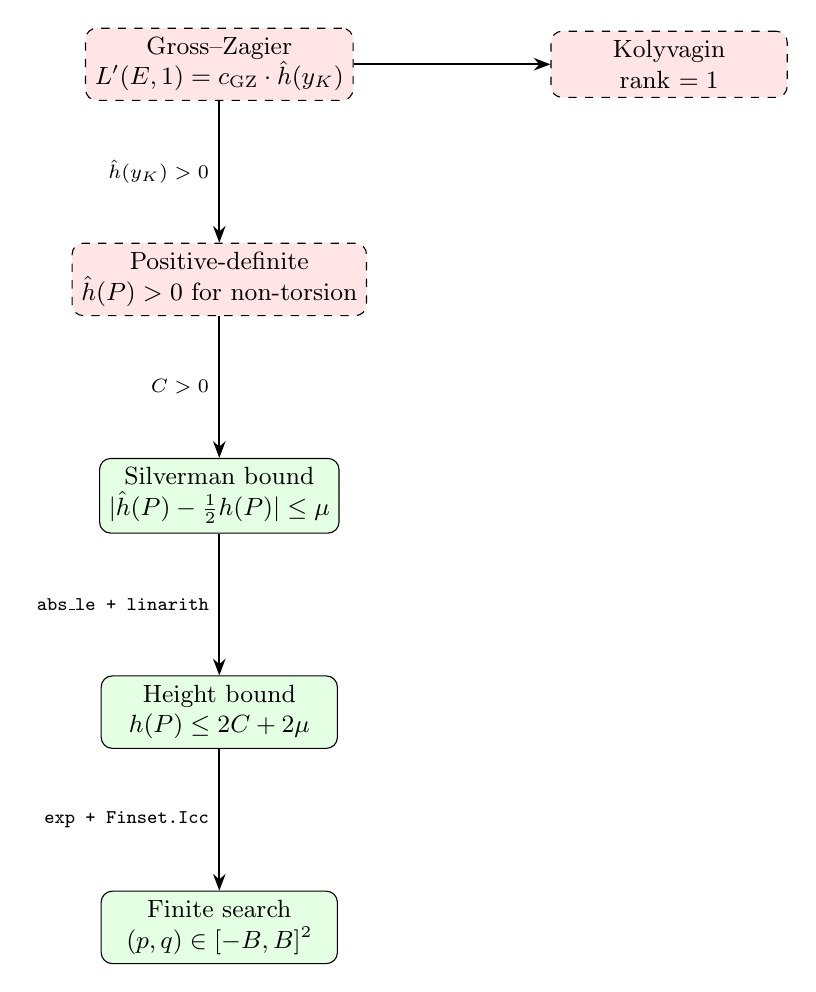
\begin{tikzpicture}[
  node distance=1.8cm,
  box/.style={rectangle, draw, rounded corners, minimum width=3cm, minimum height=0.8cm, align=center, font=\small},
  axiombox/.style={box, fill=red!10, dashed},
  bishbox/.style={box, fill=green!10},
  arrow/.style={-{Stealth[length=6pt]}, thick},
]
  \node[axiombox] (GZ) {Gross--Zagier\\$L'(E,1) = c_{\mathrm{GZ}} \cdot \hhat(y_K)$};
  \node[axiombox, right=2.5cm of GZ] (Kol) {Kolyvagin\\rank $= 1$};
  \node[axiombox, below=of GZ] (PD) {Positive-definite\\$\hhat(P) > 0$ for non-torsion};
  \node[bishbox, below=of PD] (SB) {Silverman bound\\$|\hhat(P) - \frac{1}{2}h(P)| \le \mu$};
  \node[bishbox, below=of SB] (HB) {Height bound\\$h(P) \le 2C + 2\mu$};
  \node[bishbox, below=of HB] (FS) {Finite search\\$(p,q) \in [-B,B]^2$};

  \draw[arrow] (GZ) -- node[left,font=\scriptsize] {$\hhat(y_K) > 0$} (PD);
  \draw[arrow] (PD) -- node[left,font=\scriptsize] {$C > 0$} (SB);
  \draw[arrow] (SB) -- node[left,font=\scriptsize] {\texttt{abs\_le + linarith}} (HB);
  \draw[arrow] (HB) -- node[left,font=\scriptsize] {\texttt{exp + Finset.Icc}} (FS);
  \draw[arrow] (GZ) -- (Kol);
\end{tikzpicture}
\end{center}

\noindent
\textcolor{red!60!black}{Dashed red}: axiomatized (LPO-dependent).
\textcolor{green!60!black}{Solid green}: proved ($\BISH$).

The \emph{chokepoint} between axiomatized and proved is the real-valued
Silverman bound: everything above is deep analytic number theory
(Langlands, Gross--Zagier, Kolyvagin); everything below is explicit
algebra and combinatorics.

\subsection{Classical.choice audit}\label{sec:classical-choice}

\texttt{Classical.choice} appears in the \texttt{\#print axioms} output of every theorem that operates over~$\RR$.  This is a \Mathlib{} infrastructure artifact: Lean's $\RR$ is constructed as a classical Cauchy completion, and every operation on real numbers inherits \texttt{Classical.choice}.  This is shared by \emph{all} \Mathlib{} theorems over~$\RR$, including those in Papers~23 and~28.

The constructive stratification is established by \emph{proof content}, not by the axiom checker output (see Paper~10, \S Methodology):
\begin{itemize}
  \item The BISH half (height bound chain, finite grid membership) uses only \texttt{abs\_le}, \texttt{linarith}, and \texttt{Finset.Icc}---no omniscience principle.
  \item The axiomatized half (Gross--Zagier, Kolyvagin, Silverman, positive-definiteness) enters through \texttt{Prop}-valued structure fields, not \texttt{Classical.dec}.
  \item Three theorems (\texttt{bish\_decidable\_of\_bound}, \texttt{height\_bound\_monotone}, \texttt{height\_bound\_nonneg}) depend on \emph{no axioms at all}, not even infrastructure.
\end{itemize}

\subsection{Reproducibility}\label{sec:reproducibility}

The full Lean~4 project is archived on Zenodo:
\begin{center}
DOI: \href{https://doi.org/10.5281/zenodo.18732168}{10.5281/zenodo.18732168}
\end{center}
\begin{itemize}
  \item \textbf{Lean toolchain:} \texttt{leanprover/lean4:v4.28.0-rc1}
  \item \textbf{Build command:} \texttt{lake build}
  \item \textbf{Expected output:} 0 errors, 0 warnings, 0 \texttt{sorry}
  \item \textbf{Axiom verification:} uncomment \texttt{\#print axioms} lines in \texttt{Main.lean}
\end{itemize}

% ====================================================================
\section{CRM Audit}\label{sec:crm-audit}
% ====================================================================

\subsection{Constructive strength classification}

\begin{center}
\begin{tabular}{llccc}
\toprule
\textbf{Result} & \textbf{Strength} & \textbf{Sorries} & \textbf{Custom axioms} & \textbf{Necessary?} \\
\midrule
Thm~A (BISH core + Archimedean rescue) & $\BISH$ & 0 & 0 & Yes \\
Thm~B ($p$-adic failure) & $\BISH$ & 0 & 0 & --- (negative) \\
Thm~C (Rescue gap) & $\BISH$ & 0 & 0 & --- \\
Thm~D (Axiom budget) & --- & --- & --- & (meta-analysis) \\
\bottomrule
\end{tabular}
\end{center}

All four quarantined analytic inputs (Gross--Zagier, Kolyvagin, Silverman, positive-definiteness) enter as \texttt{Prop}-valued structure fields, not as Lean \texttt{axiom} declarations.  The constructive core is pure $\BISH$.

\subsection{Comparison with Paper~45 calibration pattern}

Paper~45 (Weight-Monodromy Conjecture) established the de-omniscientizing descent pattern: abstract $\LPO$ descends to geometric $\BISH$ when the conjecture provides algebraic origin.  Paper~48 (BSD) calibrated the BSD conjecture at the abstract level, identifying $\LPO$ for the $L$-value zero-test.

Paper~51 applies the DPT framework to the \emph{same} conjecture (BSD) and finds:
\begin{itemize}
  \item \textbf{What descends:} the generator search (from $\MP$ to $\BISH$).
  \item \textbf{Mechanism:} Archimedean polarization (DPT Axiom~3), via positive-definite N\'eron--Tate height.
  \item \textbf{Where it descends from/to:} $\MP$ (unbounded search) $\to$ $\BISH$ (bounded finite grid).
  \item \textbf{Why $p$-adic fails:} $u(\QQ_p) = 4$, so positive-definiteness is absent.
\end{itemize}

This confirms the DPT prediction from Paper~50: Axiom~3 (Archimedean polarization) is the unique modality that enables descent for BSD, and its absence at finite primes explains the $p$-adic obstruction.

% ====================================================================
\section{Discussion}\label{sec:discussion}
% ====================================================================

\subsection{Connection to de-omniscientizing descent}\label{sec:descent}

Papers~45--49 calibrated five arithmetic geometry conjectures and discovered a uniform pattern: each conjecture asserts that continuous data over complete fields ($\LPO$-dependent) descends to discrete algebraic data ($\BISH$-decidable).  Paper~50 distilled this into three DPT axioms.

Paper~51 instantiates the pattern for BSD at the \emph{constructive level}: the generator search is an instance of the de-omniscientizing descent where the descent mechanism is Axiom~3 (Archimedean polarization).  The $p$-adic failure (Theorem~B) shows the descent \emph{failing} when Axiom~3 is absent---giving a concrete, machine-checked example of a blocked de-omniscientizing descent.

\subsection{The $p$-adic exceptional zero: a logical re-reading}\label{sec:exceptional}

The exceptional zero pathology of $p$-adic BSD (Mazur--Tate--Teitelbaum~\cite{mazurtate}) is usually explained analytically: trivial zeros of $p$-adic $L$-functions, extra Euler factors at~$p$.  Paper~51 gives a \emph{logical} explanation: the $p$-adic canonical height is not positive-definite, so the $\MP \to \BISH$ conversion fails.  The search remains unbounded not because of analytic complications but because the metric lacks the topological property needed for logical reduction.

The formalization makes this precise: \texttt{padic\_failure\_vacuous} shows the bound collapses to $h(P) \le 2\mu(E)$ (vacuous); \texttt{archimedean\_rescue\_gap} quantifies the gap as $2\hhat(y_K) > 0$.  This re-reading of a classical analytic obstruction as a failure of logical reducibility is, to our knowledge, new.

\subsection{Relation to other papers in the series}\label{sec:relation}

Paper~51 is the first application of constructive reverse mathematics to a Clay Millennium Problem.  It identifies the BSD analogue of the $\FT \leftrightarrow \mathrm{CompactOptimization}$ equivalence (Paper~23~\cite{paper23}): the Archimedean metric is the topological modality that converts $\MP$-level search to $\BISH$-level computation.  Like Paper~28's stratification of classical mechanics~\cite{paper28}, the constructive content is architectural---identifying the exact axiom/theorem boundary---but the subject matter (a Millennium Problem) and the logical re-reading of the exceptional zero pathology are distinctive.

\subsection{Open questions}\label{sec:open}

\begin{enumerate}
  \item Can the axiom budget be reduced further?  Specifically, does the Silverman bound follow from Gross--Zagier + Kolyvagin + a weaker height comparison?
  \item For rank~$\ge 2$, the generator search requires $\MP$ (Minkowski's second theorem gives covolume bounds but not individual basis vectors).  Can effective versions of Lang's Height Lower Bound Conjecture~\cite{lang83} gate this from $\MP$ to $\BISH$?  (Addressed in Paper~61.)
  \item The formalization covers rank~1.  Extending to rank~0 ($L(E,1) \ne 0$, which is $\BISH$ by direct evaluation) would complete the rank stratification.  (Addressed in Paper~60.)
\end{enumerate}

% ====================================================================
\section{Conclusion}\label{sec:conclusion}
% ====================================================================

Paper~51 is, to our knowledge, the first machine-checked formalization of any
component of the BSD conjecture pipeline.  It formally verifies, in
\Lean{} + \Mathlib{}, that the rank-1 BSD generator search is
$\BISH$-decidable: given quarantined analytic axioms, the search is confined
to an explicit finite grid.

The Archimedean positive-definiteness of $\hhat$ is identified as the unique
topological property enabling this reduction.  Over $\QQ_p$,
positive-definiteness fails and the search remains at the $\MP$ level---giving
a logical, not merely analytic, explanation of the exceptional zero pathology
(Mazur--Tate--Teitelbaum).

The formalization is complete with zero \texttt{sorry}s, zero custom axiom
declarations, and a clean axiom audit.  It serves as the master architecture
for a formally verified BSD solver: the deep analytic theorems (Gross--Zagier,
Kolyvagin, Silverman) interface with type theory through a single chokepoint,
and everything below that chokepoint is constructively verified.  The axiom
budget is minimal---removing any ingredient breaks the proof chain---characterizing
the necessary logical interface between analytic number theory and formal
verification.

% ====================================================================
\section{Acknowledgments}\label{sec:ack}
% ====================================================================

The author thanks the \Mathlib{} community~\cite{mathlib} for the formalization infrastructure.  Lean~4 formalization was assisted by Claude (Anthropic, Claude Code with Opus~4).  The author is a cardiologist, not a professional number theorist or logician; errors of mathematical taste or attribution are the author's responsibility.  This work is dedicated to Errett Bishop and the constructive mathematics community.

% ====================================================================
% References
% ====================================================================
\begin{thebibliography}{99}

\bibitem{silverman1}
J.\,H.~Silverman,
\emph{The Arithmetic of Elliptic Curves},
Graduate Texts in Mathematics 106, Springer, 2nd ed., 2009.

\bibitem{silverman2}
J.\,H.~Silverman,
``The difference between the Weil height and the canonical height on elliptic curves,''
\emph{Math.\ Comp.}, \textbf{55}(192):723--743, 1990.

\bibitem{grosszagier}
B.\,H.~Gross and D.\,B.~Zagier,
``Heegner points and derivatives of $L$-series,''
\emph{Invent.\ Math.}, \textbf{84}(2):225--320, 1986.

\bibitem{kolyvagin}
V.\,A.~Kolyvagin,
``Finiteness of $E(\QQ)$ and Sha for a subclass of Weil curves,''
\emph{Izv.\ Akad.\ Nauk SSSR Ser.\ Mat.}, \textbf{52}(3):522--540, 1988.

\bibitem{cremona}
J.\,E.~Cremona,
\emph{Algorithms for Modular Elliptic Curves},
Cambridge University Press, 2nd ed., 1997.

\bibitem{mazurtate}
B.~Mazur, J.~Tate, and J.~Teitelbaum,
``On $p$-adic analogues of the conjectures of Birch and Swinnerton-Dyer,''
\emph{Invent.\ Math.}, \textbf{84}(1):1--48, 1986.

\bibitem{bishop}
E.~Bishop and D.~Bridges,
\emph{Constructive Analysis},
Grundlehren der mathematischen Wissenschaften 279, Springer, 1985.

\bibitem{bridges-richman}
D.~Bridges and F.~Richman,
\emph{Varieties of Constructive Mathematics},
London Mathematical Society Lecture Note Series 97, Cambridge University Press, 1987.

\bibitem{neron}
A.~N\'eron,
``Quasi-fonctions et hauteurs sur les vari\'et\'es ab\'eliennes,''
\emph{Ann.\ of Math.}~(2), \textbf{82}:249--331, 1965.

\bibitem{lang83}
S.~Lang,
\emph{Fundamentals of Diophantine Geometry},
Springer, 1983.

\bibitem{lam}
T.\,Y.~Lam,
\emph{Introduction to Quadratic Forms over Fields},
Graduate Studies in Mathematics 67, AMS, 2005.

\bibitem{david-philippon}
S.~David and P.~Philippon,
``Minorations des hauteurs normalis\'ees des sous-vari\'et\'es de vari\'et\'es ab\'eliennes,''
\emph{Contemp.\ Math.}, \textbf{210}:333--364, 1998.

\bibitem{paper23}
P.\,C.-K.~Lee,
``Fan Theorem $\leftrightarrow$ Compact Optimization: Constructive Reverse Mathematics,''
Paper~23, CRM Series, 2026.
DOI: \href{https://doi.org/10.5281/zenodo.18604312}{10.5281/zenodo.18604312}.

\bibitem{paper28}
P.\,C.-K.~Lee,
``Newton vs.\ Lagrange vs.\ Hamilton: Constructive Stratification of Classical Mechanics,''
Paper~28, CRM Series, 2026.
DOI: \href{https://doi.org/10.5281/zenodo.18616620}{10.5281/zenodo.18616620}.

\bibitem{paper48}
P.\,C.-K.~Lee,
``Birch and Swinnerton-Dyer Conjecture and LPO,''
Paper~48, CRM Series, 2026.
DOI: \href{https://doi.org/10.5281/zenodo.18683400}{10.5281/zenodo.18683400}.

\bibitem{mathlib}
The Mathlib Community,
``Mathlib4: Mathematics in Lean 4,''
\url{https://github.com/leanprover-community/mathlib4}, 2024--2026.

\bibitem{Paper50}
P.\,C.-K.~Lee,
``Three Axioms for the Motive: A Decidability Characterization of Grothendieck's Universal Cohomology,''
Paper~50, CRM Series, 2026.
DOI: \href{https://doi.org/10.5281/zenodo.18705837}{10.5281/zenodo.18705837}.

\bibitem{Paper52}
P.\,C.-K.~Lee,
``Decidability Transfer via Specialization: Standard Conjecture~D for Abelian Threefolds,''
Paper~52, CRM Series, 2026.
DOI: \href{https://doi.org/10.5281/zenodo.18732559}{10.5281/zenodo.18732559}.

\bibitem{Paper53}
P.\,C.-K.~Lee,
``The CM Decidability Oracle: Verified Computation from Elliptic Curves to the Fourfold Boundary,''
Paper~53, CRM Series, 2026.
DOI: \href{https://doi.org/10.5281/zenodo.18713089}{10.5281/zenodo.18713089}.

\end{thebibliography}

\end{document}

